\chapter{Creación de recursos de prueba}

Con el objetivo de determinar una línea base para la creación del corpus, se inicia realizando una segmentación de recursos abiertos existentes para medir posteriormente la calidad de las segmentaciones automáticas.

Se define segmentación del audio como el proceso por el cual, a partir de una grabación de voz, se particiona la misma en segmentos mas pequeños, siendo particiones a nivel de declaración, palabra o fonético. Las anotación es el proceso por el cual a partir de una grabación de voz se relaciona el contenido linguístico de la misma

Se realizaron dos anotaciones para el desarrollo de la investigación: una anotación a nivel fonético y otra a nivel de declaración.

Para ambas anotaciones se utilizó el software Praat \cite{Praat} desarrollado por Paul Boersma y David Weenink de la Universidad de Ámsterdam. Con el cual de manera visual es posible crear archivos de anotación del audio. Estos archivos usan el formato TextGrid, especificado por la misma herramienta, donde se definen secuencias de elementos que identifican el inicio, finalización y texto encontrado en cada segmento. Estos archivos son almacenados en formato de texto para su fácil lectura \cite{TextGrids}.

Aunque en la literatura no se define con claridad los tamaños los conceptos de gran vocabulario y larga duración. Los valores considerados para este trabajo serán de 5000 palabras para un corpus de gran vocabulario y larga duración un corpus de 100 horas.

\section{Anotación manual a nivel fonético}



Las grabaciones seleccionadas para el corpus fonético de prueba se extrajeron del Open Speech Corpus \cite{Collazos2015} y el subcorpus de palabras aisladas, el cual está compuesto por 334 palabras distintas grabadas por múltiples locutores con un total de 9441 grabaciones de 39 locutores distintos, seleccionando aleatoriamente 100 palabras distintas y realizando una anotación manual por medio de PRAAT \cite{Praat}.

La anotación se realizó utilizando la convención definida en la tabla \ref{tab:anotacion_fonetica}. Esta convención se us\'o considerando que las grabaciones seleccionadas fueron grabadas en su totalidad por locutores latino americanos, del país Colombia y la región del Valle del Cauca. 

\begin{table}[H]
\centering
\caption{Anotación Fonética}
\label{tab:anotacion_fonetica}
\begin{tabular}{|l|l|l|}
\textbf{Simbolo} & \textbf{Letra} & \textbf{Representación} \\ \hline
sil              & & Silencio                               \\ \hline
a                & a & vocal open central                   \\ \hline
b                & b &  consonante plosiva bilabial sonora   \\ \hline 
k                & c &  consonante plosiva palatal no sonora \\ \hline 
S                & ch &  consonante fricativa palatal        \\ \hline 
d                & d &  consonante plosiva dental sonora     \\ \hline 
e                & e &  vocal semi-open central              \\ \hline
f                & f &  consonante fricativa labiodental     \\ \hline 
g                & g &  consonante plosiva velar sonora      \\ \hline
i                & i &  vocal closed front                   \\ \hline
j                & j &  consonante approximant palatal       \\ \hline
l                & l &  consonante approximant alveolar      \\ \hline 
m                & m &  consonante nasal bilabial            \\ \hline 
n                & n &  consonante nasal alveolar            \\ \hline 
N                & ñ &  consonante nasal palatal             \\ \hline 
o                & o &  vocal semi-closed back               \\ \hline
p                & p &  consonante plosiva no sonora         \\ \hline 
R                & r &  consonante vibrant alveolar sonora   \\ \hline 
r                & r &  consonante vibrant alveolar no sonora \\ \hline
s                & s &  consonante fricativa alveolar         \\ \hline
t                & t &  consonante plosiva dental no sonora   \\ \hline
u                & u &  vocal closed back                    \\ \hline
y                & y &  consonante fricativa palatal         \\ \hline
\end{tabular}
\end{table}

La distribución de fonemas en la anotación manual se muestra en la tabla \ref{tab:distribucion_fonetica}

\begin{table}[H]
\centering
\caption{Distribución fonética}
\label{tab:distribucion_fonetica}
\begin{tabular}{|l|l|}
\textbf{Fonema} & \textbf{Ocurrencias} \\ \hline
sil & 173 \\ \hline
a   & 91  \\ \hline
o   & 79  \\ \hline
e   & 59  \\ \hline
n   & 45  \\ \hline
i   & 40  \\ \hline
l   & 31  \\ \hline
s   & 29  \\ \hline
t   & 27  \\ \hline
d   & 22  \\ \hline
R   & 22  \\ \hline
b   & 20  \\ \hline
r   & 19  \\ \hline
p   & 19  \\ \hline
j   & 16  \\ \hline
u   & 16  \\ \hline
m   & 15  \\ \hline
k   & 14  \\ \hline
g   & 11  \\ \hline
f   & 7   \\ \hline
c   & 5   \\ \hline
y   & 5   \\ \hline
C   & 2   \\ \hline
N   & 1   \\ \hline
S   & 1   \\ \hline
\end{tabular}
\end{table}

Las grabaciones seleccionadas se distribuyen entre 22 grabadas por locutores de género femenino, 68 masculinos y 10 no identificado.

En la imagen \ref{img:anotacion_fonetica_praat} se muestra la anotación fonética de una grabación que contiene la palabra arete realizada en Praat y en el archivo \ref{file:text_grid} el archivo correspondiente a la anotación fonética. En adelante se denominará a esta anotación corpus fonético de experimentación.


\begin{figure}[H]
\caption{Anotación fonética con Praat}
\label{img:anotacion_fonetica_praat}
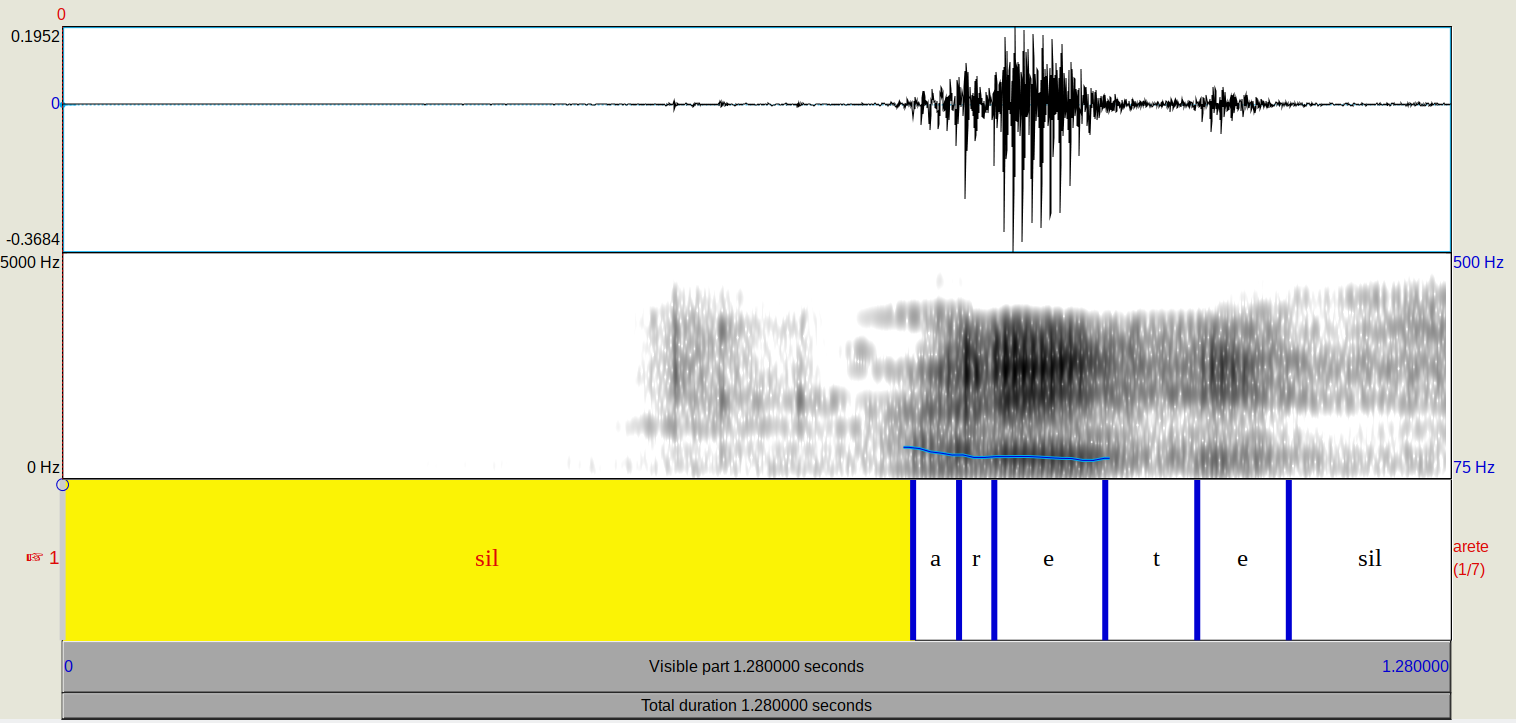
\includegraphics[width=\textwidth]{imagenes/03_01_anotacion_fonetica.png}
\end{figure}

\lstinputlisting[caption={Archivo TextGrid con anotación fonética}, label={file:text_grid}]{archivos/03_01_text_grid_ejemplo.txt}



\section{Anotación manual a nivel de sentencia}

También se realizó una anotación a nivel de declaración de los audiolibros de Librivox. Para ello se seleccionaron audios correspondiendo al 10\% del corpus, es decir, 6 horas. Sobre estos audios se realizó una segmentación manual basada en símbolos de puntuación. 

Para la selección de los audio libros, se ordenaron las grabaciones en orden ascendente considerando el tamaño del audio original en segundos, para posteriormente seleccionar 3 horas de locutores de género femenino y 3 horas del género masculino, garantizando de esta manera un balance de género y también la maximización de locutores diferentes. Cada archivo será identificado con un prefijo F o M que significa el género del locutor, separado por una línea baja \_ y el consecutivo asignado.

Los archivos almacenados en Librivox usan el formato de compresión con pérdida MP3, para su tratamiento son transformados a formato sin compresión WAV utilizando el programa Sox \cite{Sox}.

Se realizó de igual manera una descarga manual de los textos correspondientes a los audio libros seleccionados, generando archivos de texto plano cuya primera línea es el título del texto. Las líneas siguientes corresponden al texto.

Como parte del pre-procesamiento del texto, se utilizaron expresiones regulares para segmentar los textos descargados de internet por símbolos de puntuación, y generando un nuevo archivo de texto plano donde cada línea contiene un índice, y la declaración correspondiente al segmento del texto.

Se muestra un ejemplo de texto tokenizado en el archivo \ref{file:texto_tokenizado}

\lstinputlisting[caption={Texto tokenizado}, label={file:texto_tokenizado}]{archivos/03_02_tokenizacion_texto.txt}

Los índices al comienzo de cada línea funcionan como identificadores en el proceso de anotación a nivel de declaración. Esto con el objetivo de facilitar el proceso de anotación al solo indicar en el campo de texto un índice en lugar del texto correspondiente. Posteriormente es posible reconstruir un archivo de anotación, reemplazando los índices por el texto correspondiente almacenado en el archivo de tokenización. El ejemplo de anotación de declaración del texto ejemplo se puede observar en el archivo \ref{file:text_grid_tokenizado}.

\lstinputlisting[caption={Segmento de Archivo TextGrid con anotación a nivel de declaración}, label={file:text_grid_tokenizado}]{archivos/03_03_text_grid_tokenizado.txt}


En adelante se denominará a esta anotación como corpus de pruebas.

% \section{Anotación automática a nivel de sentencia usando Libri Vox Spanish}

% \textcolor{red}{WIP}

% Esta sección corresponde a la generación de TextGrids usando los archivos fuentes descargados directamente desde librivox y comparándolos con la segmentación manual de \cite{LibriVox-Spanish}, de momento no tengo nada acá mas que experimentos fallidos usando Onsets y de pronto luego miro si hay tiempo de dejar este capítulo si encuentro alguna luz. De pronto usando DTW pasa algo acá pero no se.

